\subsection{Motivación}

\begin{frame}
	\frametitle{Motivación}
	\begin{itemize}
	\item	Muchas aplicaciones de las bases de datos deben tener
		en cuenta la temporalidad de los datos. \pause
		Aplicaciones financieras, compañías de seguro, reserva
		de hoteles, registros de pacientes, sistemas de soporte
		a la decisión. \pause

	\item	Si bien se puede manejar desde un nivel mas alto, esto
		complica las consultas SQL y se vuelve inmanejable rápidamente.
		\pause

	\item	Por eso, queremos tener motores que sean ``conscientes'' de
		la temporalidad, con un lenguaje especializado.
	\end{itemize}
\end{frame}

\begin{frame}
\frametitle{Definición de DB Temporal}
	\begin{itemize}
	\item	Una DB Temporal es una DB con soporte interno para manejar
		datos temporales. \pause

	\item	Existen 3 tipos: \pause
		\begin{itemize}
		\item Histórica: mantiene el tiempo validez \pause
		\item Rollback: mantiene el tiempo de transacción \pause
		\item Bitemporales: mantiene ambos \pause
		\end{itemize}

	\item	A su vez, pueden implementarse con timestamps por tupla
		o por atributo. COMPARAR.
	\end{itemize}
\end{frame}

\begin{frame}
\frametitle{Tiempo de transacción y tiempo de validez}
	\begin{itemize}
	\item	El tiempo de {\bf validez} indica cuando una entrada de la DB
		tiene validez en la realidad que se modela. \pause Puede
		ser un intervalo completamente en el pasado, del pasado al
		futuro, o en el futuro enteramente.
	\pause
	\item	El tiempo de {\bf transacción} indica cuando la tupla se añadió
		a la DB cómo válida, y cuando se dejó de creer en su validez.
		\pause Esto permite saber que es lo que la DB ``creía'' en
		un momento determinado del pasado.
		\pause Nunca puede haber un tiempo futuro.
	\end{itemize}
\end{frame}

\begin{frame}
\frametitle{Tiempo de transacción y tiempo vaĺido}
	\begin{itemize}
	\item	Los tiempos de validez y de transacción están en dos escalas
		completamente distintas. \pause
		Si estamos modelando eventos del siglo 18, los tiempos de validez
		irán del 1700 al 1799. \pause
		Sin embargo, los de transacción irán de la fecha de creación
		de la DB hasta el presente.
	\end{itemize}
\end{frame}

\begin{frame}
	\begin{center}
	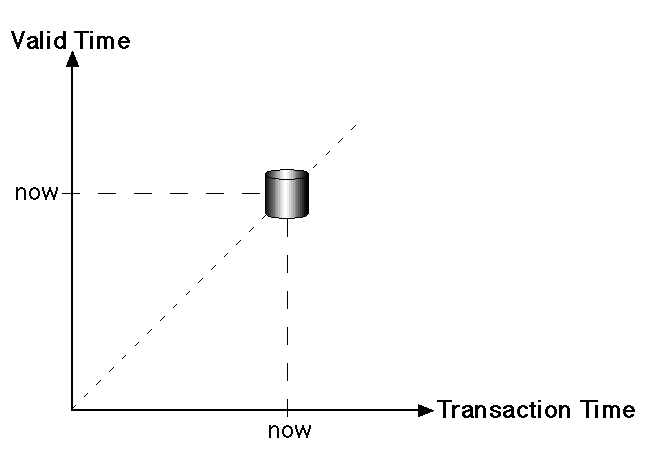
\includegraphics[height=5cm]{snapshot.png}
	\end{center}
\end{frame}

\begin{frame}
	\begin{center}
	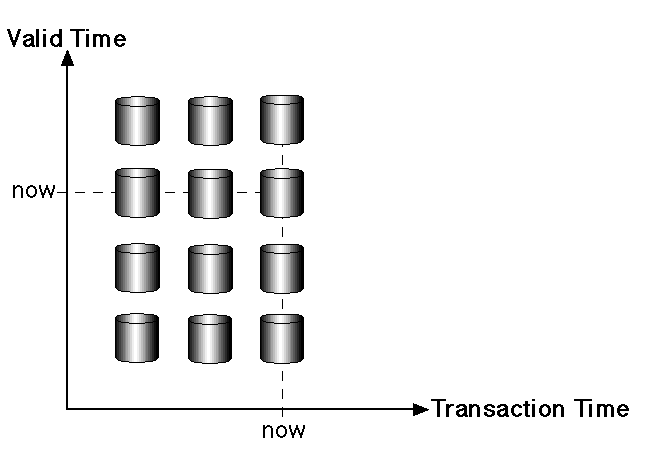
\includegraphics[height=5cm]{bitemporal.png}
	\end{center}
\end{frame}

\begin{frame}
\begin{center}
\frametitle{Ejemplo de bitemporalidad}
	\tiny

	``Desde el 1/6/1995 al 3/9/2000 John se mudó a Beachy, pero para no
	pagar impuestos, nuncá lo reportó. Luego, durante una investigación
	se descubre (en el 2/2/2001) que si se había mudado.''

	\pause
	\vspace{5mm}

	Histórica: \hfill
	\begin{tabular}{|c|c|c|c|}
	\hline
	Nombre   & Ciudad	& ValidFrom	& ValidTo	\\ \hline
	John Doe & Smallville	& 3/4/1975	& 26/8/1994	\\ \hline
	John Doe & Bigtown	& 26/8/1994	& 1/6/1995	\\ \hline
	John Doe & Beachy	& 1/6/1995	& 3/9/2000	\\ \hline
	John Doe & Bigtown	& 3/9/2000	& 1/4/2001	\\ \hline
	\end{tabular}

	\pause
	\vspace{5mm}

	\newcommand{\z}[0]{\alert<4>}

	Bitemporal: \hfill
	\begin{tabular}{|c|c|c|c|c|c|}
	\hline
	Nombre   & Ciudad	& ValidFrom	& ValidTo	& TransFrom	& TransTo	\\ \hline
	John Doe & Smallville	& 3/4/1975	& ∞		& 4/4/1975	& 27/12/1994	\\ \hline
	\z{John Doe} & \z{Smallville}	& \z{3/4/1975}	& \z{26/8/1994}	& \z{27/12/1994}	& \z{∞}	\\ \hline
	John Doe & Bigtown	& 26/8/1994	& ∞		& 27/12/1994	& 2/2/2001	\\ \hline
	\z{John Doe} & \z{Bigtown}	& \z{26/8/1994}	& \z{1/6/1995}	& \z{2/2/2001}	& \z{∞}	\\ \hline
	\z{John Doe} & \z{Beachy}	& \z{1/6/1995}	& \z{3/9/2000}	& \z{2/2/2001}	& \z{∞}	\\ \hline
	John Doe & Bigtown	& 3/9/2000	& ∞		& 2/2/2001	& 1/4/2001	\\ \hline
	\z{John Doe} & \z{Bigtown}	& \z{3/9/2000}	& \z{1/4/2001}	& \z{1/4/2001}	& \z{∞}	\\ \hline
	\end{tabular}
\end{center}
\end{frame}

\begin{frame}
\frametitle{Comparación de tipos de DB Temporal}
	\begin{figure}

	\psmatrix[mnode=r,colsep=1,rowsep=1]
	& [name=1] Bitemporal & \\
	[name=2] Histórica & & [name=3] Rollback \\
	& [name=4] Snapshot &
	\endpsmatrix
	\ncline{<-}{1}{2}
	\ncline{<-}{1}{3}
	\ncline{<-}{2}{4}
	\ncline{<-}{3}{4}
	\end{figure}
\end{frame}
